\documentclass[a4paper,12pt]{article}
\usepackage [utf8x]{inputenc}
\usepackage[czech]{babel} 
\usepackage{graphicx}
\usepackage{amsmath}
\usepackage{xspace}
\usepackage{url}
\usepackage{indentfirst}
\usepackage[margin=22mm]{geometry}
\usepackage{esvect}
\usepackage{ragged2e}
\usepackage{tikz,pgf}
\usepackage{bm}
\usepackage{perpage}
\usepackage{capt-of}
\usepackage{hyperref}
\usepackage{subcaption}
\usepackage{siunitx}

\hypersetup{
	colorlinks=true,
	filecolor=magenta,      
	urlcolor=cyan,
}

\graphicspath{
	{img/}
	{plots/}
	{imgpdf/}
	}

\MakeSorted{figure}
\newtoks\jmenopraktika \newtoks\jmeno \newtoks\datum
\newtoks\obor \newtoks\skupina \newtoks\rocnik \newtoks\semestr
\newtoks\cisloulohy \newtoks\jmenoulohy
\newtoks\tlak \newtoks\teplota \newtoks\vlhkost
\jmenopraktika={Skenovací elektronový mikroskop}  
% nahradte jmenem vaseho predmetu
\jmeno={Radek Horňák}            
\datum={14.~února 2023}        % nahradte datem mereni ulohy
\obor={F}                     
\skupina={Středa 10:00}            
\rocnik={2.}                  
\semestr={IV.}                 
\cisloulohy={6}    % cislo ulohy           

\begin{document}
	\begin{center}
		{\Large Přírodovědecká fakulta Masarykovy univerzity} \\
		\bigskip
		{\Large \bfseries EXPERIMENTÁLNÍ METODY 2} \\
		\bigskip
		{\Large \the\jmenopraktika}
	\end{center}
	\bigskip
	\noindent
	\setlength{\arrayrulewidth}{1pt}
	\begin{tabular*}{\textwidth}{@{\extracolsep{\fill}} l l}
		\large {\bfseries Zpracoval:}  \the\jmeno \hspace{40mm} \large  
		{\bfseries Datum:} \the\datum\\ \\
		\hline
	\end{tabular*}
	
	\section{Úvod}\noindent
Skenovací elektronový mikroskop (SEM) je mikroskop využívající fokusovaný 
paprsek elektronů. Cílem této úlohy je pochopit základní pojmy a principy a 
seznámit se s měřením osobně.
%\par Mezi důležité pojmy SEM je rozlišení spojené s vlnovou délkou, a tedy 
%přímo úměrné energii elektronu.
%\par V teorii jsme se seznámili s důležitými pojmy mikroskopie: rozlišení, 
%optické vady,

\section{Měření}
\subsection{Titanová tříska}\noindent
Prvním měřením bylo sledování povrchu třísky titanu po obrábění. Morfologii 
povrchu vidíme na obrázku \ref{fig:ti5000}. Snímky byly 
pořízeny při pracovní vzdálenosti (WD) 15,00\,\si{\milli\meter}, urychlovacím 
napětí 6\,\si{\kilo\volt} a zvětšení $500\times$, respektive $5000\times$. 
Vlevo vidíme snímek pořízený SE detektorem, který snímá sekundární elektrony. 
Tyto elektrony jsou generovány z malé hloubky vzorku, typicky několik 
nanometrů, 
a nesou informaci o struktuře povrchu. Na pravé straně je snímek pořízený BSE 
detektorem snímající zpětně odražené elektrony. Pravděpodobnost zpětného 
odražení je úměrná hmotnosti atomu. Tyto snímky nám tedy poskytují informaci o 
rozložení chemických prvků ve vzorku, kde světlejší místa odpovídají těžším 
prvkům.

Pro přesnější určení prvků je použita metoda energiově disperzní 
spektroskopie (EDX). Zde detekujeme rentgenové záření emitované ze vzorku, viz 
obr.~\ref{fig:EDX} a \ref{fig:EDX_tot}. 
Následně z čar charakteristického rentgenového záření jsme schopni určit 
procentuální zastoupení jednotlivých prvků. Tuto analýzu vidíme na 
obr.~\ref{fig:spectrum}. Pozorujeme kromě titanu (32,4\,\si{\percent}) také 
uhlík (52,9\,\si{\percent}), kyslík (10,5\,\si{\percent}) a hliník 
(2,7\,\si{\percent}). Na obr.~\ref{fig:EDX_C} lze vidět, že detekovaný uhlík 
kopíruje morfologii 
obrábění. Obrábění titanu je kvůli jeho tvrdosti a nízké tepelné vodivosti 
náročné, proto se musí intenzivně chladit a lubrikovat. Tyto chladiva a 
lubrikanty obsahují organické sloučeniny a vysvětlují přítomnost detekovaného 
uhlíku. 
%Nelze také vyloučit, že obráběcí nástroj je tvořen z karbidu. Mezi časté tvrdé 
%materiály obráběcích nástrojů patří také sloučeniny karbidu.


\begin{figure}[h!]
	\centering
	%\vspace*{-8mm}
	\includegraphics[width=\textwidth]{ti_500x_15mm.pdf}
	\includegraphics[width=\textwidth]{ti_5000x_15mm.pdf}
	%\vspace*{-2mm}
	\caption{\centering Morfologie povrchu titanové třísky: vlevo SE detektor, 
	vpravo BSE 
	detektor, nahoře zvětšení $500\times$, dole zvětšení $5000\times$.}
	\label{fig:ti5000}
\end{figure}


%\begin{figure}[h!]
%	\centering
%	%\vspace*{-8mm}
%	\includegraphics[width=\textwidth]{Electron Image 5.pdf}
%	%\vspace*{-2mm}
%	\caption{\centering }
%	\label{fig:Iab}
%\end{figure}

\begin{figure}[h!]
	\centering
	\begin{subfigure}{0.49\textwidth}
		%\vspace*{-8mm}
		\includegraphics[width=\textwidth]{C Kα1_2 Map Data 5.pdf}
		%\vspace*{-2mm}
		\caption{\centering C K$\alpha_{1,2}$}
		\label{fig:EDX_C}
	\end{subfigure}
	\begin{subfigure}{0.49\textwidth}
		%\vspace*{-8mm}
		\includegraphics[width=\textwidth]{Ti Lα1,2 Map Data 5.pdf}
		%\vspace*{-2mm}
		\caption{\centering Ti L$\alpha_{1,2}$}
		\label{fig:EDX_Ti}
	\end{subfigure}
	\begin{subfigure}{0.49\textwidth}
		%\vspace*{-8mm}
		\includegraphics[width=\textwidth]{O Kα1 Map Data 5.pdf}
		%\vspace*{-2mm}
		\caption{\centering O K$\alpha_{1}$}
		\label{fig:EDX_O}
	\end{subfigure}
	\begin{subfigure}{0.49\textwidth}
		%\vspace*{-8mm}
		\includegraphics[width=\textwidth]{Al Kα1 Map Data 5.pdf}
		%\vspace*{-2mm}
		\caption{\centering Al K$\alpha_{1}$}
		\label{fig:EDX_Al}
	\end{subfigure}
	
	\caption{Prvkové rozložení ve vzorku určené EDX detektorem.}
	\label{fig:EDX}
\end{figure}

\begin{figure}[h!]
	\centering
	%\vspace*{-8mm}
	\includegraphics[width=\textwidth]{EDS Layered Image 5.pdf}
	%\vspace*{-2mm}

	\begin{subfigure}{0.2\textwidth}
		\vspace*{-60mm}
		\hspace*{65mm}
		
\includegraphics[width=\textwidth]{legend.png}
	\end{subfigure}
	\caption{\centering Rozložení prvků Ti, Al a C ve vzorku.}
	\label{fig:EDX_tot}
\end{figure}

\begin{figure}[h!]
	\centering
	%\vspace*{-8mm}
	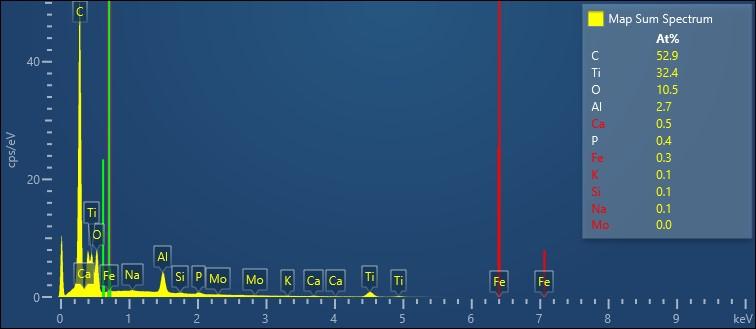
\includegraphics[width=\textwidth]{Map Sum Spectrum.jpeg}
	%\vspace*{-2mm}
	\caption{\centering Prvková analýza s procentuálním zastoupením.}
	\label{fig:spectrum}
\end{figure}

\subsection{Ubrousek a netkaná textilie}\noindent
Dále jsme sledovali vzorky ubrousku z papíru a netkané textilie a rozdíly mezi 
nimi, viz obr.~\ref{fig:ubrousek} a \ref{fig:uterka}. Jelikož se 
jedná o nevodivé vzorky, museli jsme je napřed pokovit tenkou vrstvou v 
magnetronové naprašovačce. Na obr.~\ref{fig:uterka} při zvětšení $500\times$ 
vidíme místa, kde se pokovení neuchytilo. Dochází zde k lokálnímu nabíjení 
vzorku, což způsobuje rozmazání snímku a~sníží jeho kvalitu. Chybějící vrstva 
lze také 
vidět při použitém BSE 
detektoru -- pokovení je zpravidla z těžkých kovů jako např. zlato nebo 
paladium a 
tyto prvky jde vidět jasněji na BSE detektoru než prvek netkané textilie -- 
uhlík.

\begin{figure}[h!]
	\centering
	%\vspace*{-8mm}
	\includegraphics[width=\textwidth]{ubrousek_200x_44mm.pdf}
	\includegraphics[width=\textwidth]{ubrousek_500x_44mm.pdf}
	%\vspace*{-2mm}
	\caption{\centering Morfologie povrchu ubrousku: vlevo SE detektor, vpravo 
	BSE 
		detektor, nahoře zvětšení $200\times$, dole zvětšení $1000\times$.}
	\label{fig:ubrousek}
\end{figure}

\begin{figure}[h!]
	\centering
	%\vspace*{-8mm}
	\includegraphics[width=\textwidth]{uterka_200x_42mm.pdf}
	\includegraphics[width=\textwidth]{uterka_500x_44mm.pdf}
	%\vspace*{-2mm}
	\caption{\centering Morfologie povrchu utěrky: vlevo SE detektor, vpravo 
	BSE detektor, nahoře zvětšení $200\times$, dole zvětšení $500\times$.}
	\label{fig:uterka}
\end{figure}

\clearpage
\section{Závěr}\noindent
V této úloze jsme se seznámili se skenovacím elektronovým mikroskopem. Naučili 
jsme se připravit, popř. pokovit vzorky a následně pracovat s přiloženým 
softwarem -- nastavit hloubku ostrosti, zaostřit a provést prvkovou analýzu 
pomocí EDX.

Pozorovanými vzorky byla titanová tříska, na které jsme pozorovali stopy 
po obrábění, včetně prvkových stop zejména uhlíku určených pomocí EDX. Poté 
jsme pozorovali rozdíly mezi papírovým ubrouskem a netkanou textilií. Papírový 
ubrousek je složen z celulózy, zatímco u netkané textilie lze vidět jednotlivá 
vlákna propletená/slisovaná mezi sebou. U~vzor\-ku netkané textilie jsme také 
pozorovali efekty nabíjení způsobené odloupnutím naprášené tenké vrstvy kovu.

%Někdo by si mohl snadno pomýlit zkratky EDX a XRD. Jsou to však velmi odlišné 
%metody. XRD (X-ray diffraction) je analytická metoda pro určení atomové a 
%molekulární struktury krystalu. Krystalová mřížka způsobí difrakci 
%dopadajícího 
%rentgenového záření. Měřením úhlů a intenzit rozptýleného záření lze určit 
%střední polohy atomů v krystalu, chemické vazby, rozměr elementární buňky aj. 
%Tato metoda je velmi špatná pro určení chemického složení, k~čemuž je užitečné 
%využít právě EDX před použitím XRD.

Někdo by si snadno mohl zaměnit zkratky EDX a XRD. Avšak jde o velmi odlišné 
metody. XRD (X-ray diffraction), tedy rentgenová difrakce, je analytická metoda 
určená pro zjišťování atomové a molekulární struktury krystalů. Krystalová 
mřížka způsobuje difrakci dopadajícího rentgenového záření. Měřením úhlů a 
intenzity rozptýleného záření lze určit střední polohy atomů v krystalu, 
chemické vazby, rozměry elementární buňky atd. Tato metoda je však velmi 
nevhodná pro určení chemického složení, pro což je užitečné využít právě metodu 
EDX před použitím XRD.


\end{document}
